% =============================================================
%  Informe Técnico — Car Damage ViT
%  Autores: Pablo Gomez, Matias Tripode
% =============================================================
\documentclass[12pt,a4paper]{article}

% --- Codificación y lenguaje ---
\usepackage[utf8]{inputenc}
\usepackage[T1]{fontenc}
\usepackage[spanish,es-tabla]{babel}

% --- Diseño de página ---
\usepackage[top=2.5cm, bottom=2.5cm, left=2.5cm, right=2.5cm]{geometry}
\usepackage{parskip}          % espacio entre párrafos en lugar de sangría

% --- Gráficos y figuras ---
\usepackage{graphicx}
\usepackage{float}
\usepackage{caption}
\usepackage{subcaption}
\graphicspath{
  {../docs/captures/}
  {../docs/architecture/}
  {figuras/}
}

% --- Tablas ---
\usepackage{booktabs}
\usepackage{array}
\usepackage{longtable}
\usepackage{xcolor}
\usepackage{colortbl}

% --- Matemáticas ---
\usepackage{amsmath}

% --- Código fuente ---
\usepackage{listings}
\lstset{
  basicstyle=\ttfamily\small,
  backgroundcolor=\color{gray!10},
  frame=single,
  breaklines=true,
  keywordstyle=\color{blue},
  commentstyle=\color{green!60!black},
  stringstyle=\color{red!70!black},
  numbers=left,
  numberstyle=\tiny\color{gray},
  xleftmargin=1.5em,
  framexleftmargin=1.5em,
}

% --- Hiperlinks ---
\usepackage{hyperref}
\hypersetup{
  colorlinks=true,
  linkcolor=blue!70!black,
  urlcolor=blue!70!black,
  citecolor=green!60!black,
}

% --- Colores personalizados ---
\definecolor{rowgray}{gray}{0.93}
\definecolor{headerblue}{RGB}{30, 90, 160}

% =============================================================
%  PORTADA
% =============================================================
\title{
  \vspace{1cm}
  {\LARGE \textbf{Car Damage ViT}} \\[0.5em]
  {\large Informe Técnico} \\[1em]
  {\normalsize Clasificación de daños en vehículos mediante Vision Transformers}
  \vspace{0.5cm}
}
\author{
  Pablo Gomez \quad \& \quad Matias Tripode \\[0.3em]
  \small Vision Por Computadora III
}
\date{Abril 2026}

% =============================================================
\begin{document}
% =============================================================

\maketitle
\thispagestyle{empty}
\vspace{1cm}

\begin{abstract}
Este informe documenta el desarrollo de un pipeline completo de clasificación de daños en
vehículos utilizando Vision Transformers (ViT). Se evaluaron dos arquitecturas ligeras ---
DeiT-tiny y MobileViT-small --- sobre el dataset CarDD, implementando una estrategia de
parches centrados en regiones de interés. El sistema resultante incluye una API REST,
una interfaz web, una app iOS y un mecanismo de retroalimentación humana (RLHF) con
persistencia en MinIO, todo orquestado mediante Docker Compose. MobileViT-small obtuvo
el mejor desempeño con 77,92\% de accuracy y 0,7596 de macro F1 en el conjunto de test.
\end{abstract}

\newpage
\tableofcontents
\newpage

% =============================================================
\section{Objetivo del Proyecto}
% =============================================================

El objetivo principal de este proyecto es construir un sistema capaz de \textbf{identificar
y clasificar automáticamente el tipo de daño presente en un vehículo} a partir de una
imagen, con el fin de acelerar los procesos de peritaje y estimación de reparaciones.

\subsection*{Objetivos específicos}
\begin{itemize}
  \item Implementar y comparar dos arquitecturas Vision Transformer ligeras:
        \textbf{DeiT-tiny} y \textbf{MobileViT-small}, adecuadas para despliegue en
        dispositivos de recursos limitados.
  \item Desarrollar una estrategia de extracción de parches centrados en bounding boxes
        (224$\times$224 px) que convierta la detección de objetos en un problema de
        clasificación de parches.
  \item Construir una API REST de producción con soporte para retroalimentación humana
        (\textit{human-in-the-loop}) y persistencia de correcciones en MinIO.
  \item Proveer interfaces de usuario accesibles: aplicación móvil iOS y dashboard web.
\end{itemize}

\subsection*{Dataset y Análisis Exploratorio}

Se utilizó el dataset \textbf{CarDD} (\textit{Car Damage Detection Dataset}), disponible
en HuggingFace. El análisis exploratorio completo fue realizado en el notebook
\texttt{01\_eda\_cardd.ipynb} (Pablo Gomez).

\textbf{Splits y volumen:}

\begin{table}[H]
  \centering
  \begin{tabular}{lrr}
    \toprule
    \textbf{Split} & \textbf{Imágenes} & \textbf{Anotaciones} \\
    \midrule
    Train       & 1.971 & 4.332 \\
    Validación  &   422 & 1.005 \\
    Test        &   423 &   874 \\
    \midrule
    \textbf{Total} & \textbf{2.816} & \textbf{6.211} \\
    \bottomrule
  \end{tabular}
  \caption{Distribución del dataset CarDD. Promedio: 2,21 instancias por imagen.}
\end{table}

Las anotaciones están en formato COCO (bounding boxes + máscaras de segmentación,
exportadas con FiftyOne). La verificación de integridad del EDA confirmó
\textbf{0 inconsistencias} entre detecciones y segmentaciones en las 2.816 imágenes.

\textbf{Distribución de instancias por clase:}

\begin{table}[H]
  \centering
  \renewcommand{\arraystretch}{1.2}
  \begin{tabular}{lrrrrr}
    \toprule
    \textbf{Clase} & \textbf{Instancias} & \textbf{\%} &
    \textbf{Small \%} & \textbf{Medium \%} & \textbf{Large \%} \\
    \midrule
    \rowcolor{rowgray}
    scratch       & 2.560 & 41,2 &  1,4 & 31,0 & 67,6 \\
    dent          & 1.806 & 29,1 &  1,7 & 15,2 & 83,1 \\
    \rowcolor{rowgray}
    crack         &   651 & 10,5 & 39,0 & 52,1 &  8,9 \\
    lamp\_broken  &   494 &  7,9 &  0,0 &  2,2 & 97,8 \\
    \rowcolor{rowgray}
    glass\_shatter&   475 &  7,6 &  0,0 &  0,4 & 99,6 \\
    tire\_flat    &   225 &  3,6 &  0,0 &  2,2 & 97,8 \\
    \midrule
    \textbf{Total} & \textbf{6.211} & 100 & & & \\
    \bottomrule
  \end{tabular}
  \caption{Distribución de instancias y escala por clase (umbrales COCO: small $<32^2$,
  medium $32^2$--$96^2$, large $\geq 96^2$ píxeles).}
\end{table}

Dos observaciones críticas para el entrenamiento:

\begin{itemize}
  \item \textbf{Desbalance severo:} scratch + dent concentran el 70,3\% de las instancias.
        tire\_flat tiene 11,4$\times$ menos instancias que scratch, lo que justifica el
        uso de \texttt{WeightedRandomSampler}.
  \item \textbf{crack es la clase más difícil:} el 39\% de sus instancias son objetos
        pequeños (small), con un área mediana de solo 6.517 px$^2$ frente a
        443.770 px$^2$ de glass\_shatter. Esto explica las confusiones observadas en la
        matriz de confusión.
\end{itemize}

\textbf{Índice de dificultad por clase} (compuesto por proporción de objetos pequeños,
ratio máscara/imagen y densidad de instancias):

\begin{table}[H]
  \centering
  \begin{tabular}{lcccc}
    \toprule
    \textbf{Clase} & \textbf{Small \%} & \textbf{Mediana máscara/imagen} &
    \textbf{Inst./imagen} & \textbf{Dificultad} \\
    \midrule
    \rowcolor{rowgray}
    crack         & 39,0 & 0,002 & 1,50 & \textbf{0,942} \\
    scratch       &  1,4 & 0,028 & 1,70 & 0,503 \\
    \rowcolor{rowgray}
    dent          &  1,7 & 0,051 & 1,45 & 0,422 \\
    lamp\_broken  &  0,0 & 0,126 & 1,01 & 0,228 \\
    \rowcolor{rowgray}
    tire\_flat    &  0,0 & 0,285 & 1,03 & 0,141 \\
    glass\_shatter&  0,0 & 0,519 & 1,01 & 0,001 \\
    \bottomrule
  \end{tabular}
  \caption{Índice de dificultad por clase. crack es la clase más desafiante;
  glass\_shatter la más fácil por su gran tamaño relativo.}
\end{table}

\textbf{Co-ocurrencia entre clases:} El par dent--scratch co-ocurre en 648 imágenes,
lo que genera confusión entre estas clases durante la clasificación. glass\_shatter
aparece aislado en la mayoría de los casos (469 imágenes propias, sin co-ocurrencia
con tire\_flat), lo que facilita su detección pero limita los ejemplos de entrenamiento
combinados.

Se agrega clase adicional \texttt{fondo} (background) durante la extracción de parches,
resultando en \textbf{7 clases totales} para el clasificador.

% =============================================================
\section{Arquitectura General}
% =============================================================

\subsection{Diagrama del sistema}

\begin{figure}[H]
  \centering
  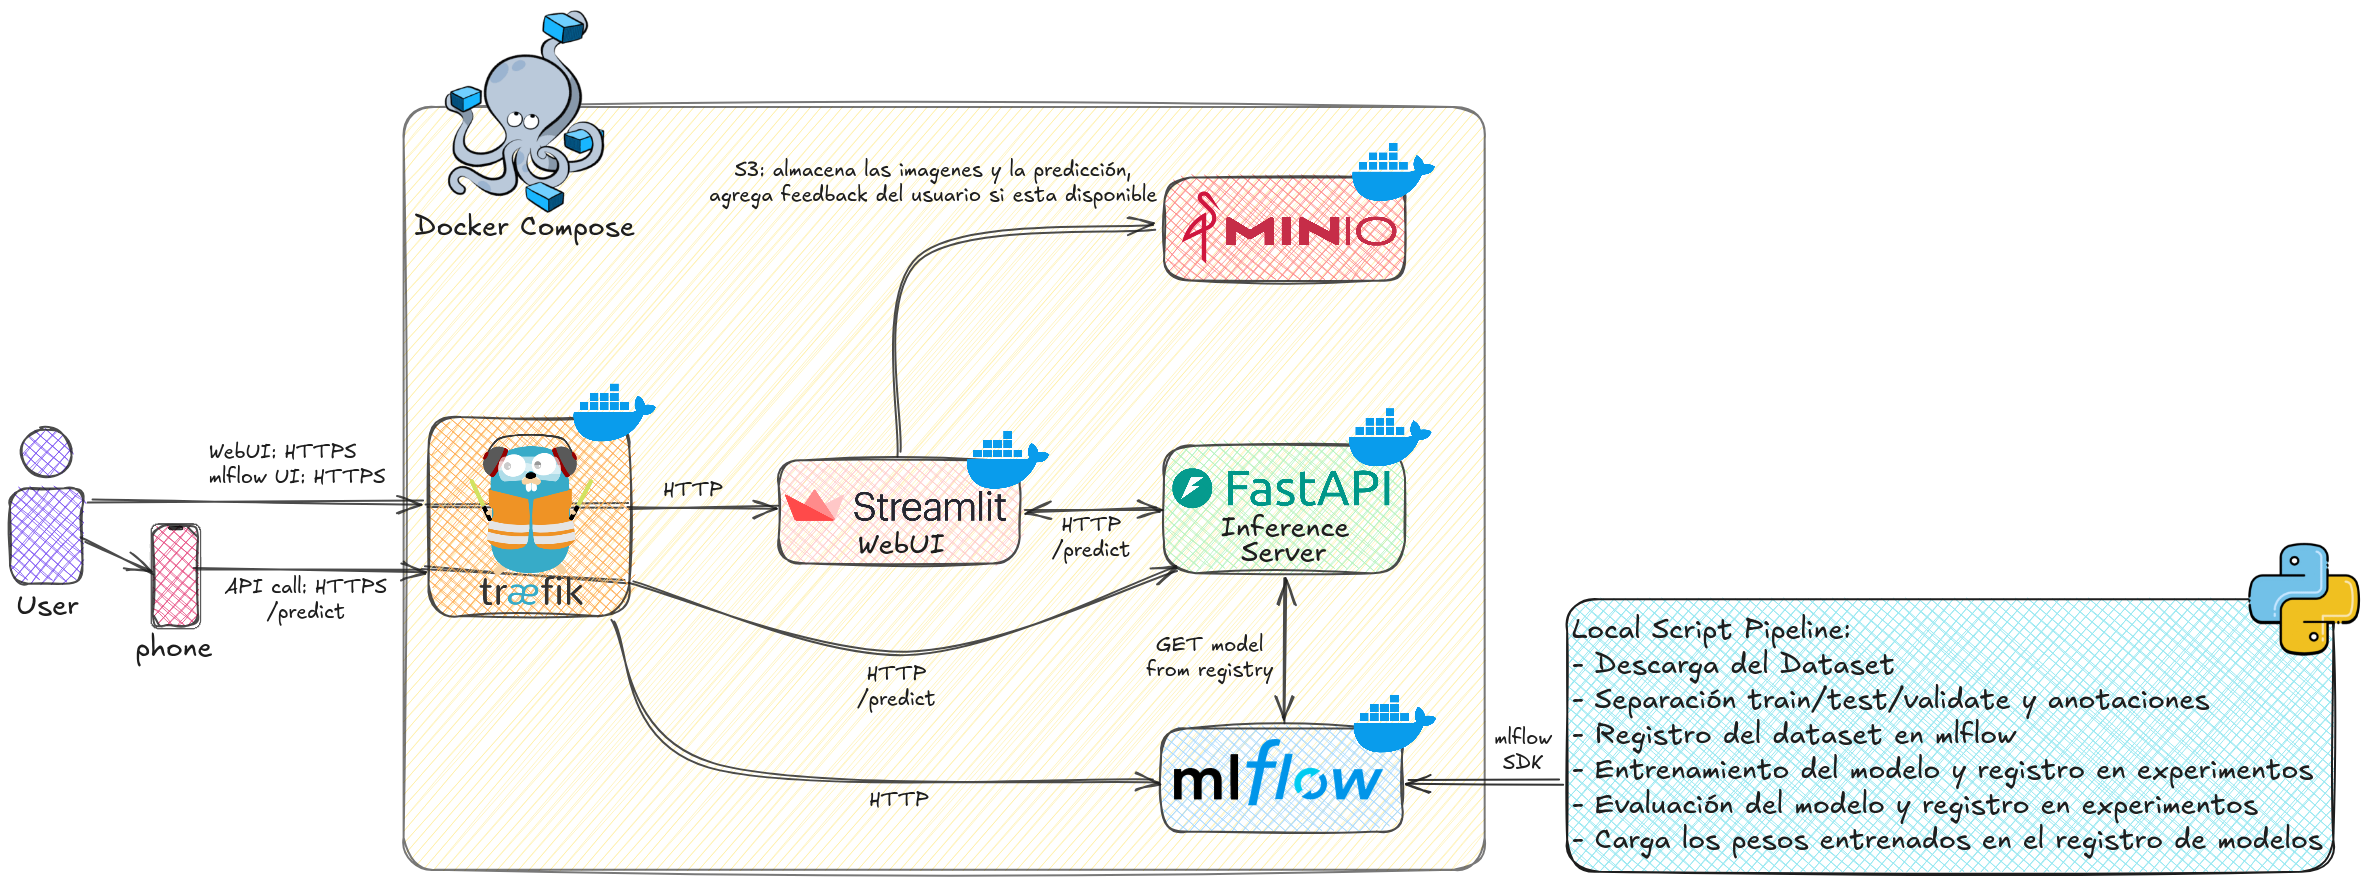
\includegraphics[width=\textwidth]{Diagrama_app.png}
  \caption{Arquitectura del sistema Car Damage ViT. El tráfico HTTPS ingresa por
  Traefik, que enruta hacia la API FastAPI y la UI Streamlit. MLflow gestiona el
  registro de modelos y MinIO almacena los datos de retroalimentación RLHF.}
\end{figure}

\subsection{Componentes del sistema}

\begin{table}[H]
  \centering
  \renewcommand{\arraystretch}{1.3}
  \begin{tabular}{p{3.2cm} p{3.8cm} p{6.5cm}}
    \toprule
    \textbf{Componente} & \textbf{Tecnología} & \textbf{Función} \\
    \midrule
    \rowcolor{rowgray}
    Reverse proxy   & Traefik v3.2           & Terminación TLS/HTTPS, routing hacia servicios internos \\
    API backend     & FastAPI + Uvicorn       & Inferencia del modelo, persistencia RLHF, hot-reload \\
    \rowcolor{rowgray}
    UI web          & Streamlit              & Selección interactiva de ROI por click, predicción y feedback humano integrado \\
    App móvil       & SwiftUI (iOS)          & Captura de imagen, envío a API, corrección humana \\
    \rowcolor{rowgray}
    Model registry  & MLflow 3.10.1          & Tracking de experimentos, versionado y aliases de modelos \\
    Object storage  & MinIO (S3-compatible)  & Persistencia de ROIs y anotaciones YOLO para RLHF \\
    \rowcolor{rowgray}
    Orquestación    & Docker Compose         & Stack completo reproducible en un único comando \\
    \bottomrule
  \end{tabular}
  \caption{Componentes del sistema y sus tecnologías.}
\end{table}

\subsection{Flujo de inferencia}

El flujo principal de una predicción sigue estos pasos:

\begin{enumerate}
  \item El usuario captura o selecciona una imagen desde la app iOS.
  \item La imagen se envía vía HTTPS al endpoint \texttt{POST /predecir}.
  \item Traefik termina TLS y reenvía la solicitud a la API FastAPI.
  \item La API extrae la región de interés (ROI 224$\times$224 px), aplica el
        procesador de imágenes y realiza inferencia con MobileViT-small.
  \item Se devuelve la clase predicha, confianza y top-3 en formato JSON.
  \item Si RLHF está habilitado, la ROI y la predicción se persisten en MinIO
        (de forma asíncrona, sin bloquear la respuesta).
\end{enumerate}

% =============================================================
\section{Implementación Técnica}
% =============================================================

\subsection{Preprocesamiento del dataset}

La estrategia central del proyecto convierte el problema de detección de objetos en
\textbf{clasificación de parches}:

\begin{itemize}
  \item Por cada anotación, se extrae un parche de 224$\times$224 px centrado en el
        bounding box (\texttt{CarDamageDataset}, \texttt{src/vit/data/dataset.py}).
  \item Se generan parches de fondo (\texttt{fondo}) con IoU = 0 respecto a cualquier
        anotación, en proporción 1:1 con los parches de daño.
  \item El desbalance de clases (tire\_flat tiene 11,6$\times$ menos instancias que
        scratch) se mitiga con \texttt{WeightedRandomSampler} en el DataLoader.
\end{itemize}

\subsection{Modelos evaluados}

\begin{table}[H]
  \centering
  \begin{tabular}{lllll}
    \toprule
    \textbf{Modelo} & \textbf{HuggingFace ID} & \textbf{Parámetros} &
    \textbf{Learning rate} & \textbf{Épocas} \\
    \midrule
    DeiT-tiny       & \texttt{facebook/deit-tiny-patch16-224} & $\sim$5,7M & 2$\times$10$^{-5}$ & 15 \\
    MobileViT-small & \texttt{apple/mobilevit-small}          & $\sim$5,6M & 1$\times$10$^{-4}$ & 15 \\
    \bottomrule
  \end{tabular}
  \caption{Configuración de los modelos evaluados. Ambos con batch size=32, weight decay=0.01,
  warmup ratio=0.1 y seed=42.}
\end{table}

Ambos modelos se cargan desde HuggingFace con \texttt{AutoModelForImageClassification},
reemplazando la cabeza de clasificación por una capa lineal de 7 salidas
(\texttt{src/vit/models/factory.py}):

\noindent\begin{minipage}{\linewidth}
\begin{lstlisting}[language=Python, caption={Carga del modelo desde HuggingFace.}]
def cargar_modelo(nombre, num_clases, attn_implementation=None):
    procesador = AutoImageProcessor.from_pretrained(nombre, use_fast=True)
    modelo = AutoModelForImageClassification.from_pretrained(
        nombre,
        num_labels=num_clases,
        ignore_mismatched_sizes=True,
        attn_implementation=attn_implementation,
    )
    return modelo, procesador
\end{lstlisting}
\end{minipage}

\subsection{Pipeline de entrenamiento}

El entrenamiento (\texttt{src/vit/train/trainer.py}) incluye:
\begin{itemize}
  \item \textbf{Early stopping} con paciencia configurable sobre val\_accuracy.
  \item \textbf{Checkpointing} del mejor modelo en \texttt{checkpoints/<modelo>/best\_model.pt}.
  \item \textbf{MLflow logging}: parámetros de configuración, métricas por época
        (loss, accuracy, macro F1) y artefactos (modelo final).
  \item Soporte de dispositivos: MPS (Apple Silicon), CUDA y CPU.
\end{itemize}

\subsection{API REST}

La API (\texttt{app/main.py}) expone tres endpoints principales:

\begin{table}[H]
  \centering
  \renewcommand{\arraystretch}{1.3}
  \begin{tabular}{p{4.5cm} p{3cm} p{6cm}}
    \toprule
    \textbf{Endpoint} & \textbf{Método} & \textbf{Descripción} \\
    \midrule
    \rowcolor{rowgray}
    \texttt{/predecir}         & POST & Recibe imagen multipart, retorna clase + confianza + top-3 \\
    \texttt{/feedback}         & POST & Corrección humana: \texttt{roi\_key} + \texttt{clase\_correcta} \\
    \rowcolor{rowgray}
    \texttt{/modelo/recargar}  & POST & Hot-reload del modelo desde MLflow Registry \\
    \bottomrule
  \end{tabular}
  \caption{Endpoints de la API FastAPI.}
\end{table}

La API utiliza \texttt{RLock} para thread safety durante la inferencia y un lock
separado para operaciones MinIO. El feedback se persiste de forma \textit{best-effort}:
un fallo en MinIO no interrumpe la predicción.

\subsection{UI Web — versión 1}

La versión 1 de la UI web (Pablo Gomez, abril 2026) introduce las siguientes mejoras
sobre la versión inicial:

\begin{itemize}
  \item \textbf{Selección de ROI por click:} se reemplazaron los sliders X/Y por
        interacción directa sobre la imagen usando \texttt{streamlit\_image\_coordinates}.
        Al hacer click, la ROI de 224$\times$224 px se centra automáticamente en el punto
        seleccionado. Los sliders quedan disponibles como ajuste fino opcional.
  \item \textbf{Feedback humano integrado (paso 3):} tras recibir una predicción, la UI
        muestra un selector de clase y un botón ``Send feedback'' que envía
        \texttt{roi\_key} + \texttt{clase\_correcta} al endpoint \texttt{/feedback},
        unificando el flujo RLHF sin necesidad de la app iOS.
  \item \textbf{Ancho máximo fijo (1024 px):} se aplica CSS personalizado para mejorar
        la legibilidad en pantallas anchas.
  \item \textbf{Gestión de estado por sesión:} se usa \texttt{st.session\_state} para
        preservar predicción y feedback entre rerenders, evitando pérdida de resultados
        al interactuar con la UI.
\end{itemize}

\subsection{Infraestructura RLHF}

Cuando el usuario corrige una predicción errónea (desde la app iOS o la UI web):
\begin{enumerate}
  \item Se envía \texttt{roi\_key} (clave del parche en MinIO) y \texttt{clase\_correcta}.
  \item La API genera una anotación en formato YOLO y la guarda junto al parche ROI
        en el bucket \texttt{rlhf} de MinIO.
  \item Estos datos quedan persistidos en MinIO y disponibles para un eventual pipeline de re-entrenamiento (fuera del alcance del presente proyecto).
\end{enumerate}

% =============================================================
\section{Evaluación: Métricas de Desempeño}
% =============================================================

\subsection{Comparación de modelos}

\begin{table}[H]
  \centering
  \renewcommand{\arraystretch}{1.4}
  \begin{tabular}{lcccc}
    \toprule
    \textbf{Modelo} & \textbf{Parámetros} &
    \textbf{Accuracy (test)} & \textbf{Macro F1 (test)} & \textbf{Resultado} \\
    \midrule
    DeiT-tiny       & $\sim$5,7M & 0,7608 & 0,7531 & \\
    \rowcolor{rowgray}
    \textbf{MobileViT-small} & \textbf{$\sim$5,6M} & \textbf{0,7792} & \textbf{0,7596} &
    \textbf{Ganador} \\
    \bottomrule
  \end{tabular}
  \caption{Resultados en el conjunto de test. MobileViT-small supera a DeiT-tiny en
  ambas métricas con un número similar de parámetros.}
\end{table}

MobileViT-small logra +1,84 pp de accuracy y +0,65 pp de macro F1 respecto a DeiT-tiny,
con prácticamente los mismos parámetros ($-$0,1M). Esta ventaja se atribuye a la
arquitectura híbrida CNN + Transformer de MobileViT, que captura mejor las características
locales relevantes para daños de pequeño tamaño.

\subsection{Curvas de entrenamiento}

\begin{figure}[H]
  \centering
  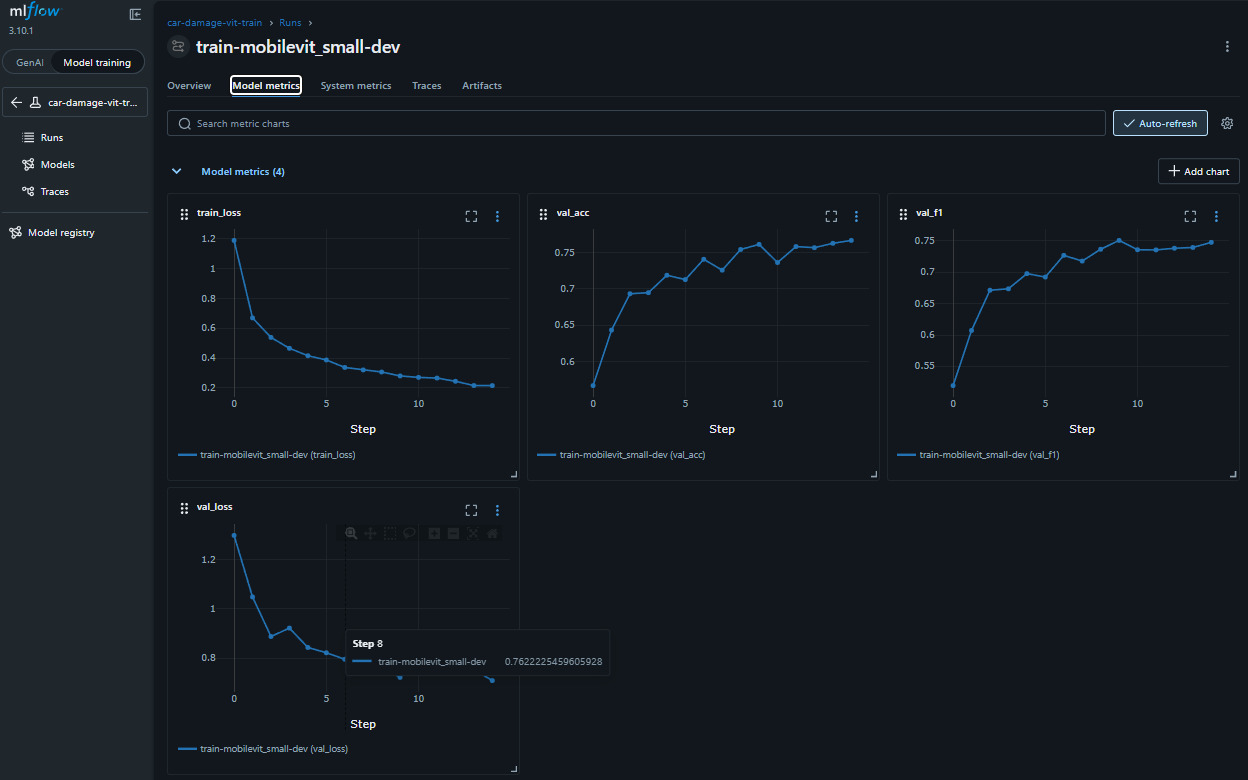
\includegraphics[width=0.95\textwidth]{model_train_graph.jpeg}
  \caption{Evolución de métricas durante el entrenamiento de MobileViT-small (15 épocas).
  El mejor checkpoint se alcanza en la época 12 con val\_accuracy=0,7624 y val\_F1=0,7451.}
\end{figure}

La pérdida de entrenamiento decrece consistentemente (1,233 → 0,223), mientras que la
pérdida de validación se estabiliza alrededor de la época 9--12, indicando que el modelo
converge sin sobreajuste severo.

\subsection{Matriz de confusión}

\begin{figure}[H]
  \centering
  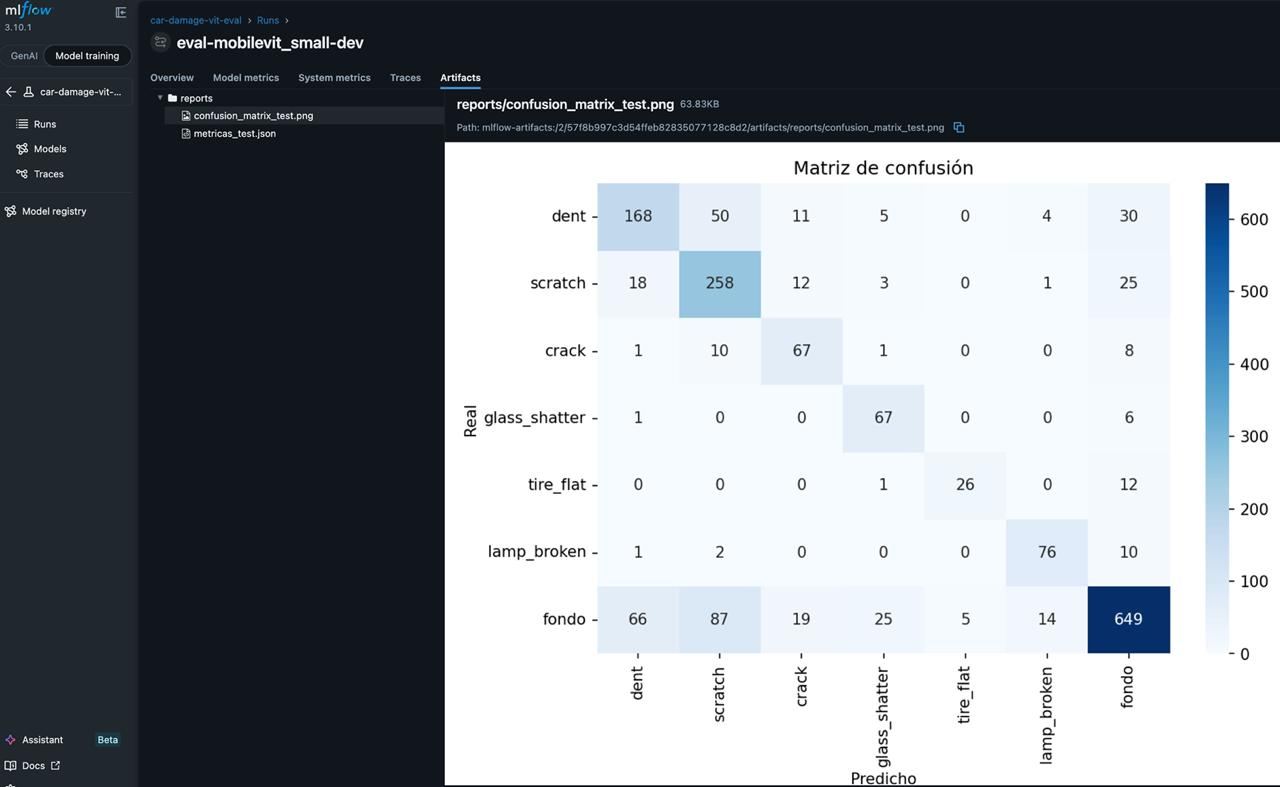
\includegraphics[width=0.75\textwidth]{confusion_matrix.jpeg}
  \caption{Matriz de confusión de MobileViT-small sobre el conjunto de test (7 clases).
  La clase \texttt{fondo} muestra el mayor número de predicciones correctas (649).
  Las mayores confusiones ocurren entre \texttt{crack}/\texttt{scratch} y
  \texttt{lamp\_broken}/\texttt{glass\_shatter}.}
\end{figure}

Observaciones clave:
\begin{itemize}
  \item \textbf{Fondo (fondo):} mejor clasificado, ya que sus parches son visualmente
        distintos a los daños.
  \item \textbf{tire\_flat} y \textbf{glass\_shatter:} mayor tasa de confusión, en parte
        por su menor representación en el dataset (desbalance de clases).
  \item \textbf{crack / scratch:} confusión frecuente por similitud visual entre ambas
        clases en parches pequeños.
\end{itemize}

% =============================================================
\section{Resultados y Ejemplos}
% =============================================================

\subsection{Visualización de atención}

Los mapas de atención permiten interpretar qué zonas de la imagen determinaron la
predicción del modelo. Se implementaron dos técnicas según la arquitectura:

\begin{itemize}
  \item \textbf{DeiT-tiny → Attention Rollout:} propaga los pesos de atención capa a
        capa multiplicando las matrices de atención con conexión residual. Los pesos de
        la fila del token CLS indican la contribución de cada parche a la predicción final.
  \item \textbf{MobileViT-small → GradCAM:} hookea la última capa del encoder para
        capturar activaciones y gradientes. Los gradientes se promedian espacialmente
        (Global Average Pooling) y se ponderan por canal para producir el mapa de calor.
\end{itemize}

Los mapas se generan con \texttt{scripts/visualizar\_atenciones.py} y se guardan en
\texttt{reports/figuras/}. En ambos modelos, las zonas de mayor activación corresponden
a la región del daño, lo que confirma que los modelos aprenden representaciones
relevantes y no artefactos espurios.

\begin{figure}[H]
  \centering
  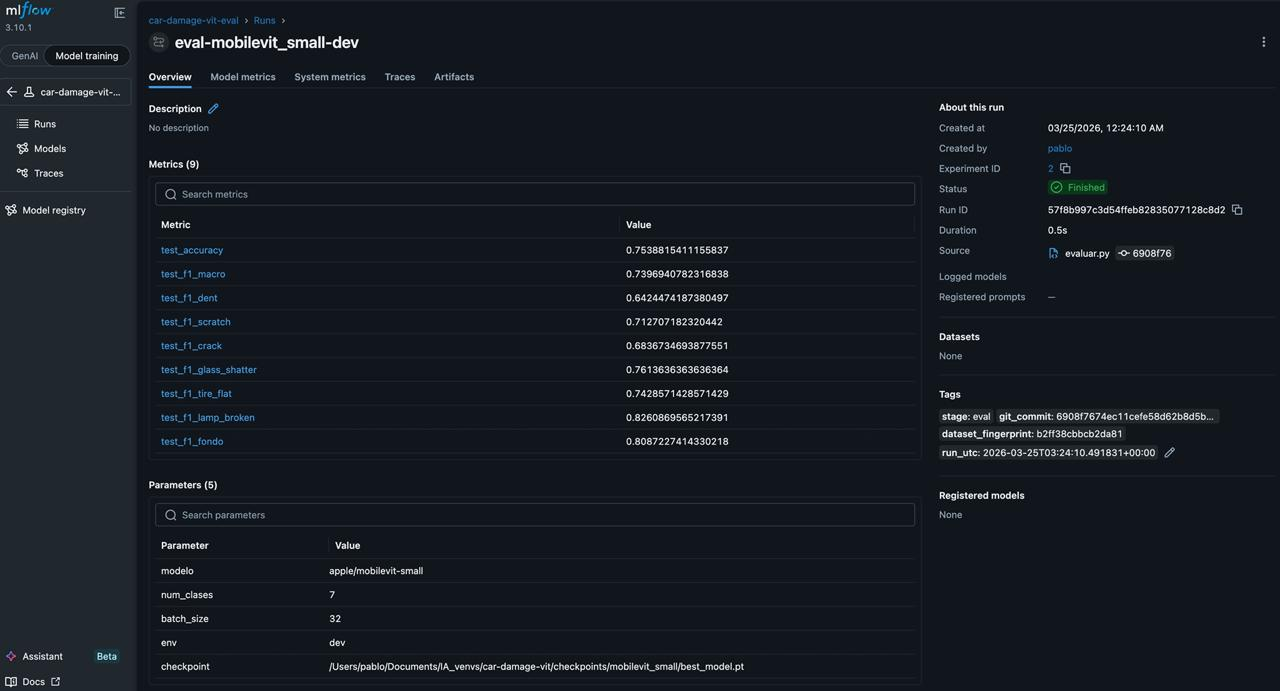
\includegraphics[width=0.85\textwidth]{model_eval.jpeg}
  \caption{Interfaz de evaluación del modelo en MLflow. Muestra las métricas de
  desempeño sobre el conjunto de test, incluyendo accuracy y macro F1 por época.}
\end{figure}

\subsection{Interfaces del sistema}

\begin{figure}[H]
  \centering
  \begin{subfigure}[b]{0.48\textwidth}
    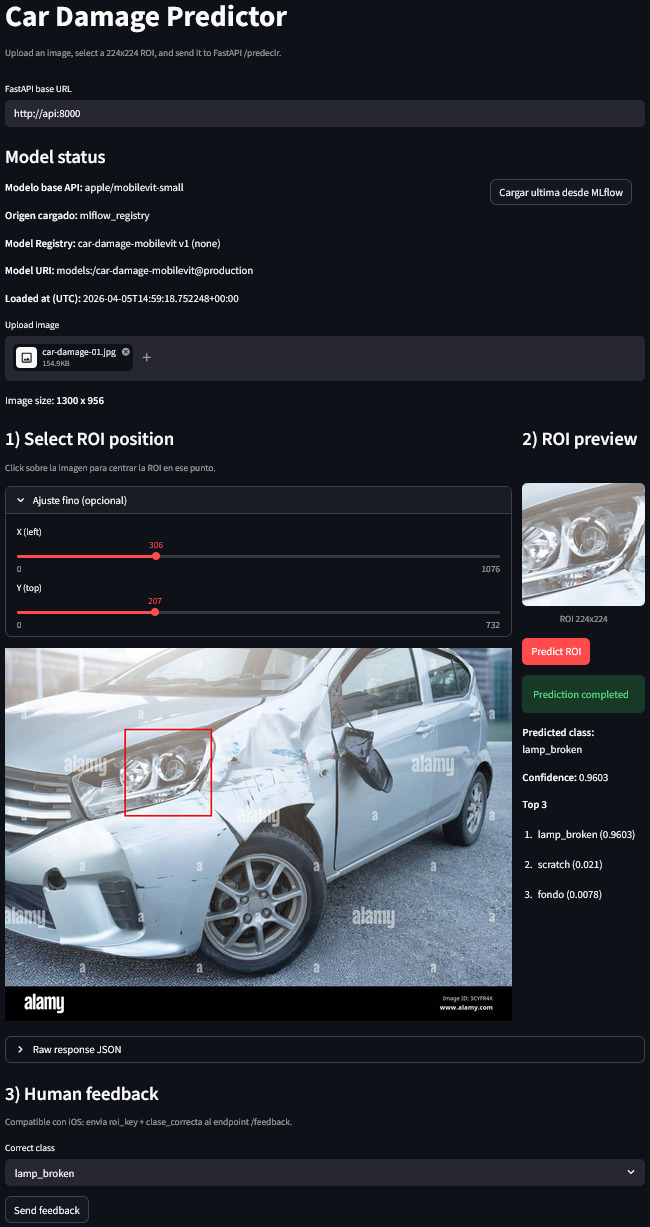
\includegraphics[width=\textwidth]{webui_v1.jpeg}
    \caption{UI web v1: selección de ROI por click sobre la imagen y resultado de predicción.}
  \end{subfigure}
  \hfill
  \begin{subfigure}[b]{0.48\textwidth}
    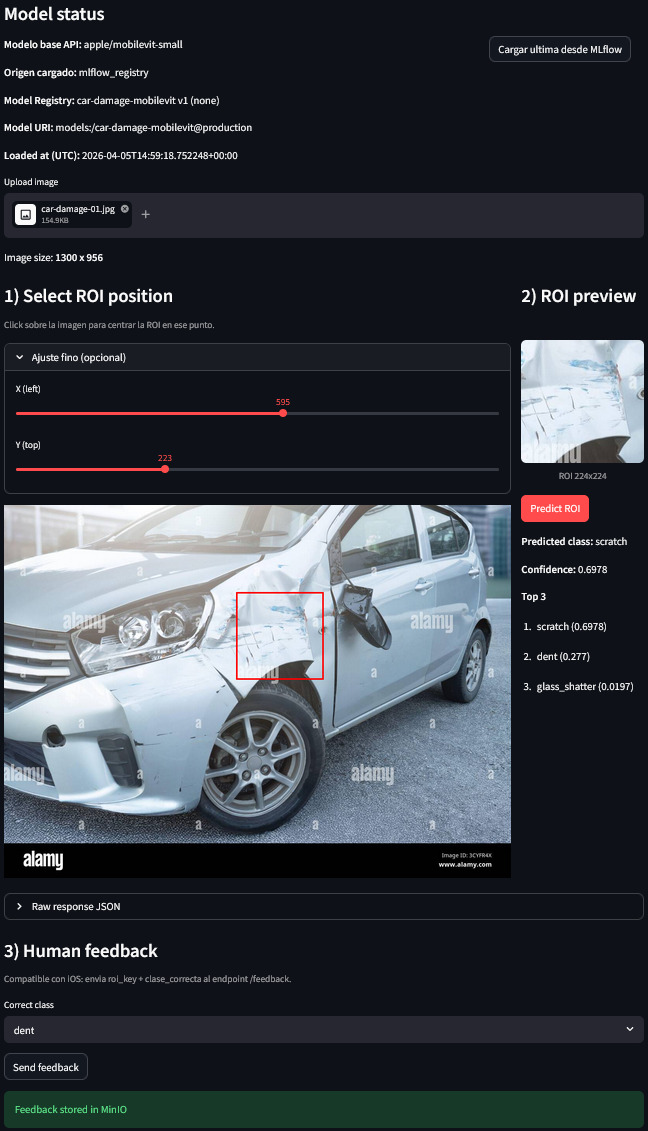
\includegraphics[width=\textwidth]{webui_v1_feedback.jpeg}
    \caption{UI web v1: sección de feedback humano integrada (paso 3).}
  \end{subfigure}
  \caption{Web UI v1. La versión actualizada reemplaza los sliders por selección
  interactiva de ROI mediante click y agrega la sección de corrección humana
  directamente en la interfaz web, unificando el flujo RLHF en un solo paso.}
\end{figure}

\begin{figure}[H]
  \centering
  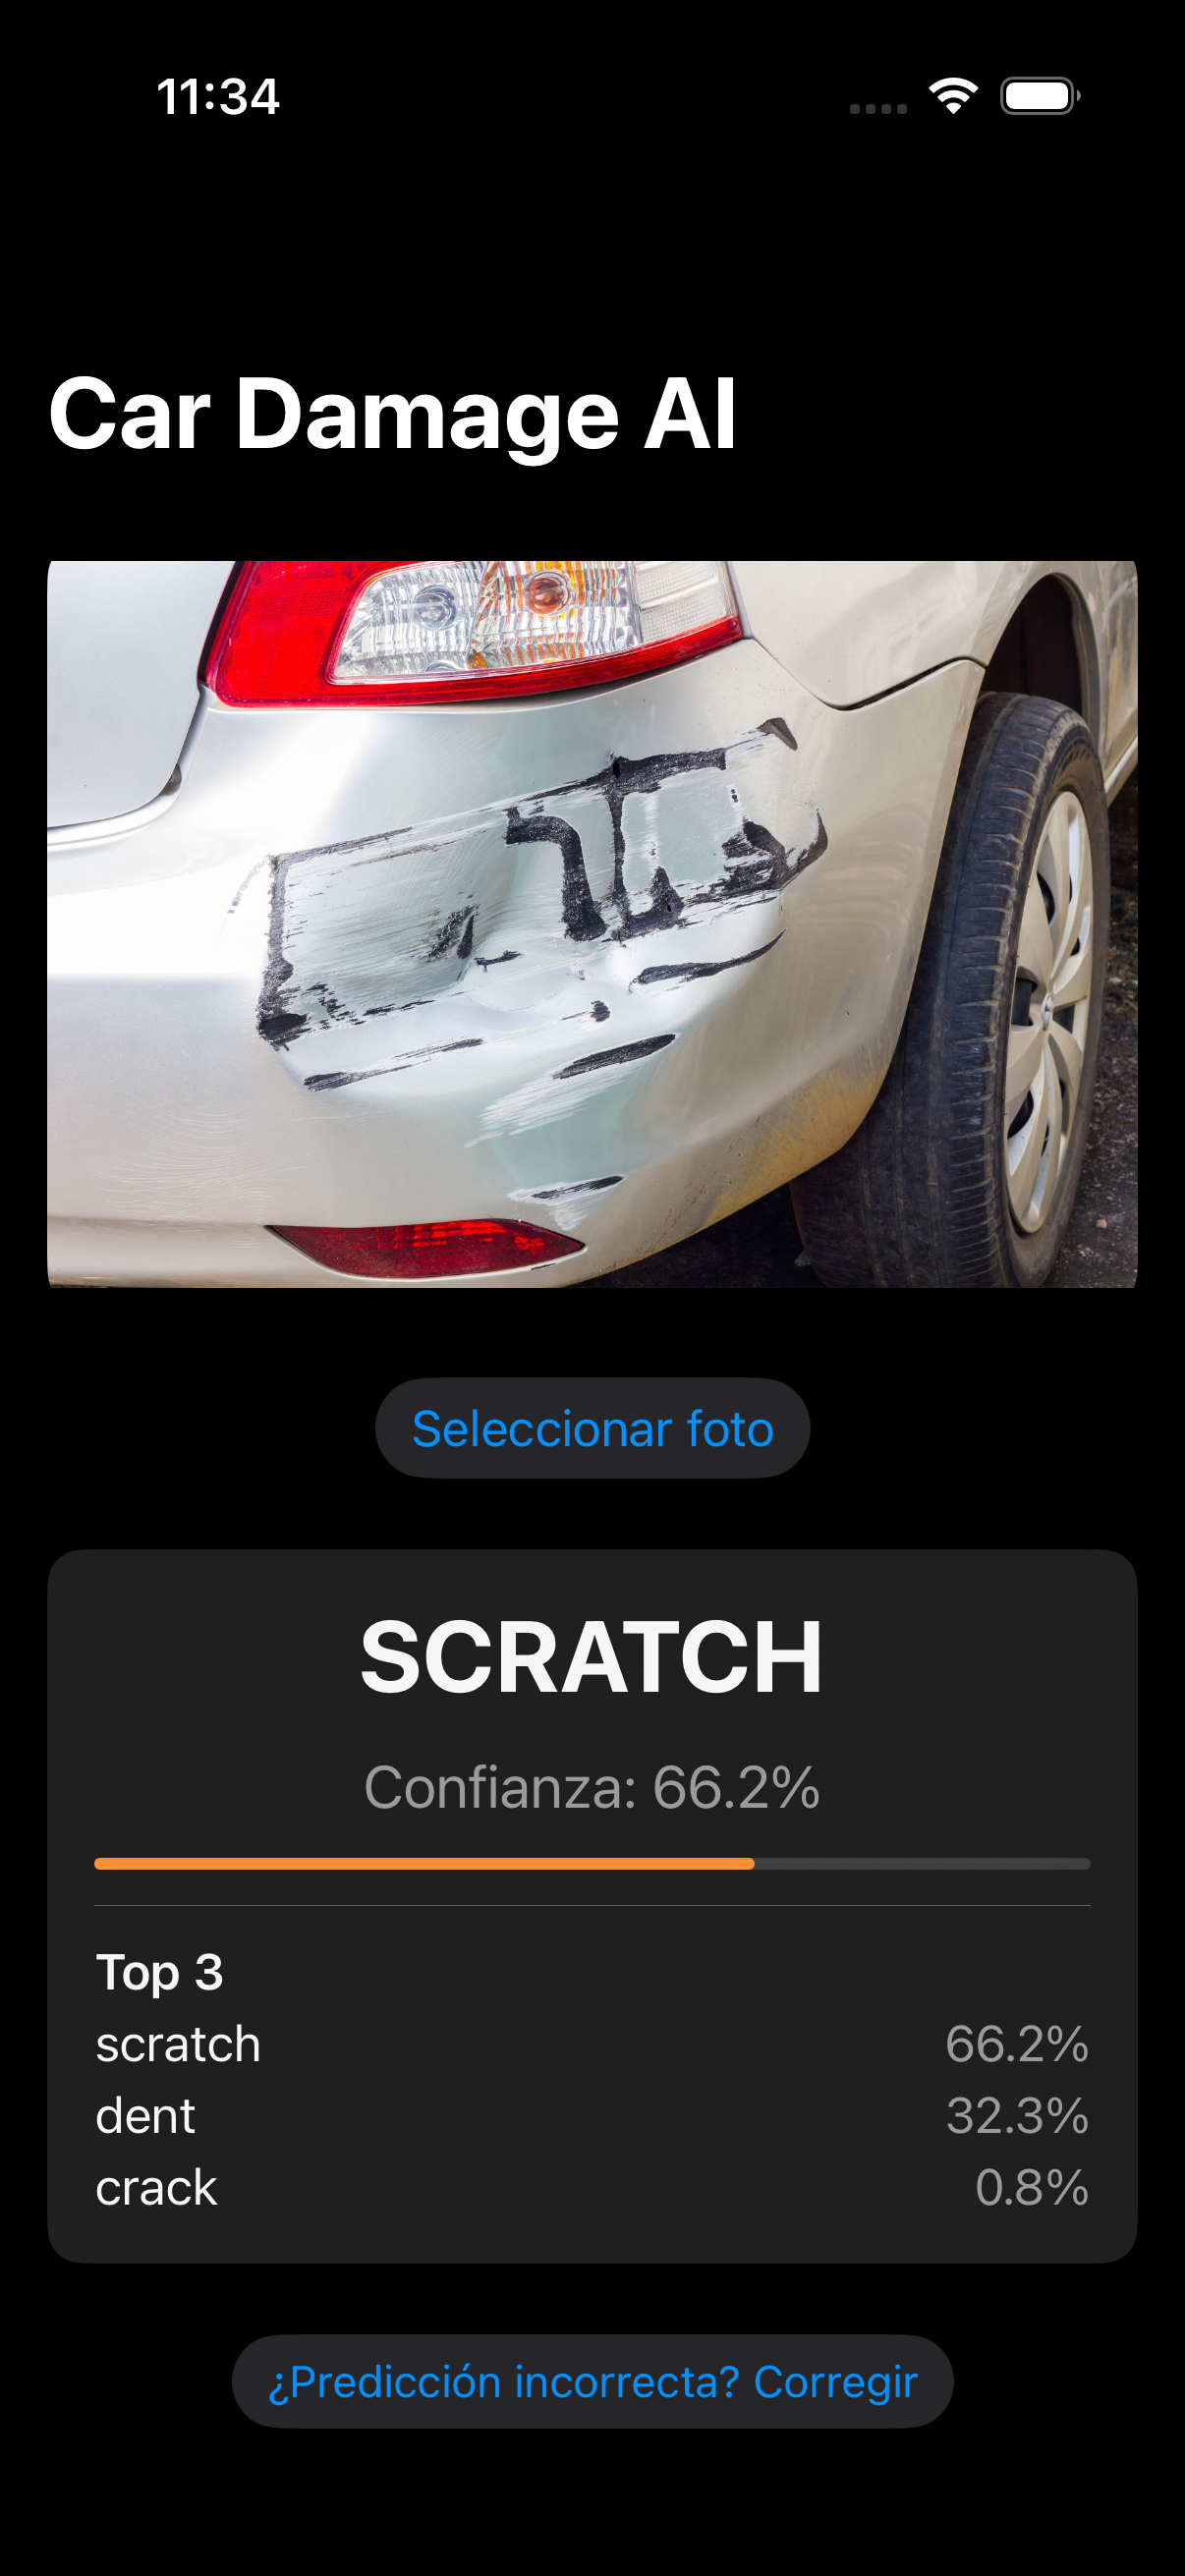
\includegraphics[width=0.45\textwidth]{phone_app.png}
  \caption{App iOS: selección de imagen y envío a la API.}
\end{figure}

\subsection{Ejemplo de respuesta de la API}

\noindent\begin{minipage}{\linewidth}
\begin{lstlisting}[language={},caption={Respuesta del endpoint \texttt{POST /predecir}.}]
{
  "clase": "scratch",
  "confianza": 0.82,
  "top3": [
    {"clase": "scratch",      "confianza": 0.82},
    {"clase": "dent",         "confianza": 0.12},
    {"clase": "crack",        "confianza": 0.04}
  ],
  "rlhf_storage": {
    "bucket": "rlhf",
    "roi_key":
      "rlhf/2026/04/04/20260404T143021123Z_abc123def456.jpg",
    "prediction_key":
      "rlhf/2026/04/04/20260404T143021123Z_abc123def456.json"
  }
}
\end{lstlisting}
\end{minipage}

\subsection{MLflow: tracking y registro de modelos}

\begin{figure}[H]
  \centering
  \begin{subfigure}[b]{0.48\textwidth}
    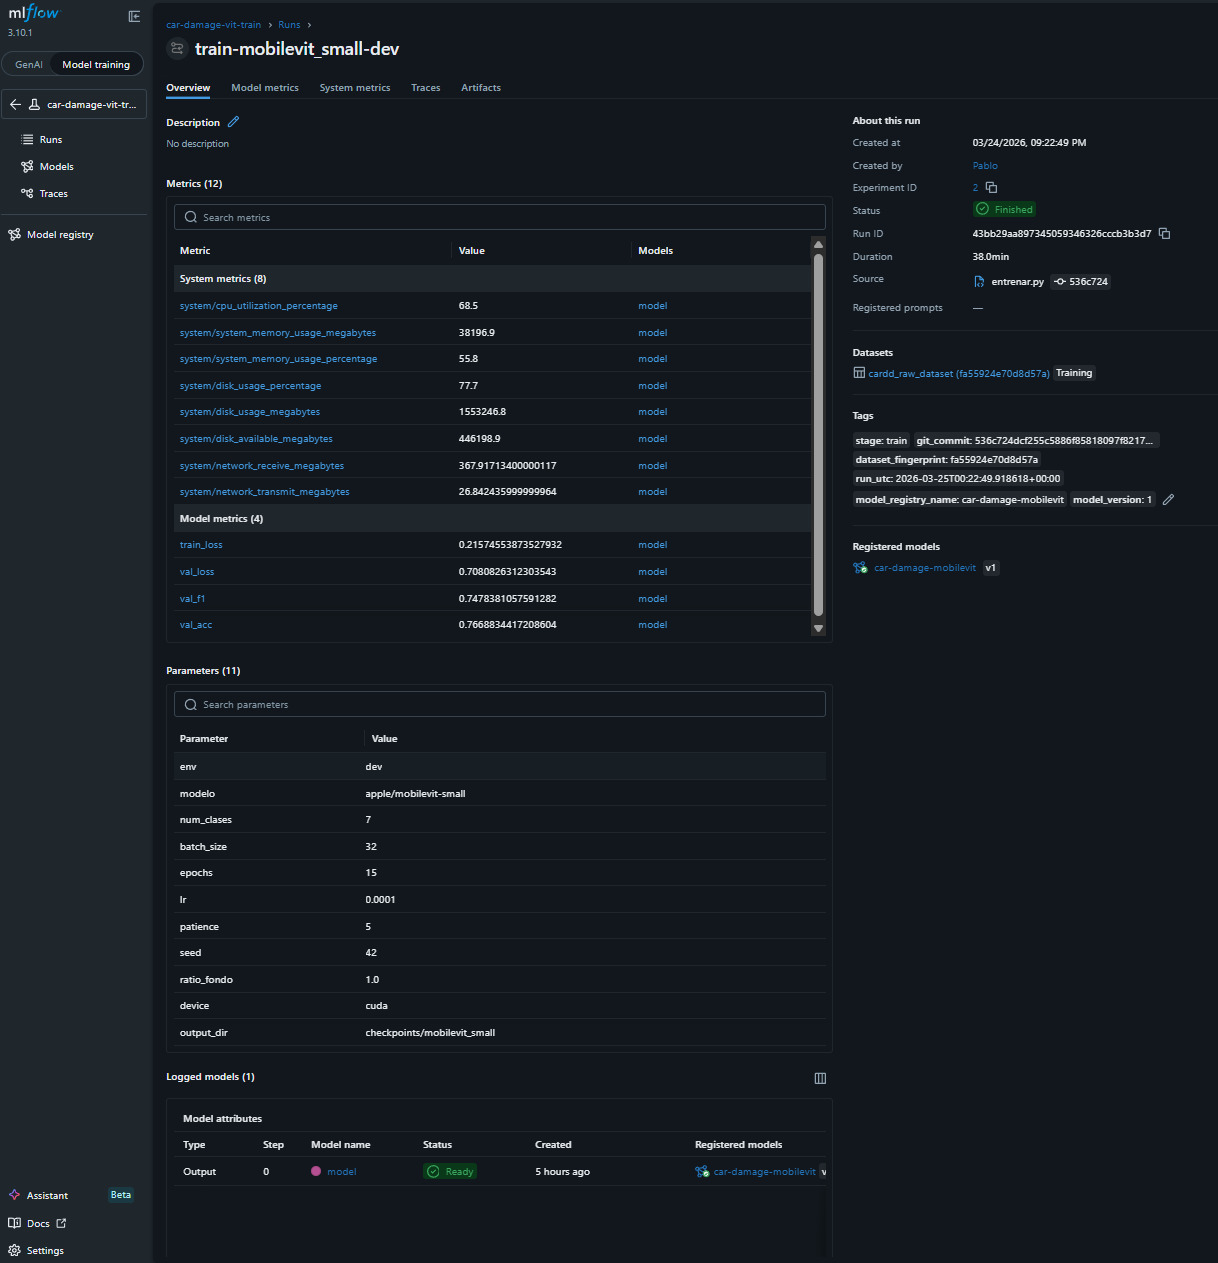
\includegraphics[width=\textwidth]{model_train.jpeg}
    \caption{Experimento de entrenamiento registrado en MLflow.}
  \end{subfigure}
  \hfill
  \begin{subfigure}[b]{0.48\textwidth}
    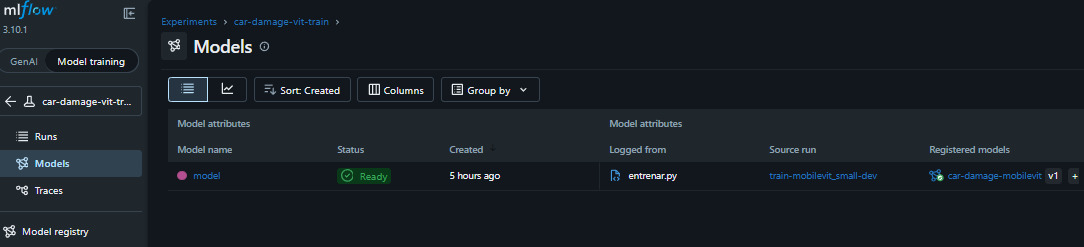
\includegraphics[width=\textwidth]{model_registry.jpeg}
    \caption{Model Registry con alias \texttt{champion}.}
  \end{subfigure}
  \caption{Interfaz de MLflow mostrando el tracking de experimentos y el registro de modelos.
  La API carga el modelo vía alias, permitiendo promoverse nuevas versiones sin reiniciar.}
\end{figure}

% =============================================================
\section{Conclusiones y Mejoras Futuras}
% =============================================================

\subsection{Conclusiones}

\begin{enumerate}
  \item \textbf{MobileViT-small es la arquitectura ganadora.} Con solo 5,6M parámetros,
        logra 77,92\% de accuracy y macro F1 de 0,7596, superando a DeiT-tiny en ambas
        métricas. Su arquitectura híbrida CNN + ViT le permite capturar mejor las
        características locales de daños pequeños.

  \item \textbf{La estrategia de parches es efectiva.} Convertir detección en clasificación
        permite reutilizar ViTs pre-entrenados en ImageNet sin necesidad de fine-tuning
        de cabezas de detección más complejas.

  \item \textbf{El pipeline end-to-end es funcional y desplegable.} Desde la captura
        móvil hasta la retroalimentación humana, el sistema opera de forma integrada
        con un único \texttt{docker compose up}.

  \item \textbf{La recolección de feedback humano está operativa.} Las correcciones
        ingresadas desde la app iOS o la UI web se persisten en MinIO como pares
        ROI + anotación YOLO. El pipeline de re-entrenamiento automático queda fuera
        del alcance de este proyecto y se propone como trabajo futuro.
\end{enumerate}

\subsection{Mejoras futuras}

\subsubsection*{Migración a segmentación de instancias con Mask2Former}

Como parte de la exploración de mejoras, se
entrenó y evaluó \textbf{Mask2Former con backbone Swin-Small}
(\texttt{facebook/mask2former-swin-small-coco-instance}) sobre el dataset CarDD durante
20 épocas, obteniendo los siguientes resultados en el conjunto de test:

\begin{table}[H]
  \centering
  \begin{tabular}{lcc}
    \toprule
    \textbf{Tarea} & \textbf{mAP @ IoU 0.50:0.95} & \textbf{mAP @ IoU 0.50} \\
    \midrule
    Bounding box (bbox)        & 0,571 & 0,706 \\
    Segmentación de instancias & 0,551 & 0,700 \\
    \bottomrule
  \end{tabular}
  \caption{Resultados de Mask2Former-Swin-Small sobre CarDD (test set, 20 épocas).}
\end{table}

Estos resultados demuestran que la arquitectura de segmentación de instancias es un
camino de mejora concreto y prometedor:

\begin{itemize}
  \item Un mAP@0.50 de \textbf{0,706 en detección} es competitivo considerando que el
        modelo no fue entrenado con datos de dominio específico.
  \item La segmentación de instancias permite delimitar con precisión el contorno del
        daño, información valiosa para estimaciones de reparación.
  \item A diferencia de la estrategia de parches actual, Mask2Former procesa la imagen
        completa en una sola pasada, eliminando la necesidad de extraer ROIs manualmente.
  \item El desempeño en objetos pequeños (AP$_\text{small}$ = 0,051) indica que el
        modelo aún tiene margen de mejora con augmentación específica y mayor resolución
        de entrada.
\end{itemize}

La integración de Mask2Former como backend de inferencia de la API representa la
\textbf{dirección de evolución prioritaria} del sistema.

\subsubsection*{Otras mejoras}

\begin{table}[H]
  \centering
  \renewcommand{\arraystretch}{1.3}
  \begin{tabular}{p{7.5cm} p{5cm}}
    \toprule
    \textbf{Mejora} & \textbf{Impacto esperado} \\
    \midrule
    \rowcolor{rowgray}
    Análisis de F1 por clase (tire\_flat, glass\_shatter) &
    Identificar clases con bajo rendimiento \\
    Fine-tuning con CLIP &
    Mayor robustez ante variaciones de dominio \\
    \rowcolor{rowgray}
    Augmentación diferencial para clases raras &
    Mejorar recall en tire\_flat y glass\_shatter \\
    Activar WeightedRandomSampler en producción &
    Mitigar desbalance de clases en el entrenamiento \\
    \rowcolor{rowgray}
    Análisis de errores: crack vs.\ scratch, lamp\_broken vs.\ glass\_shatter &
    Reducir confusiones entre clases similares \\
    Implementar tests de integración (issue \#11) &
    Mayor cobertura y confiabilidad del pipeline \\
    \rowcolor{rowgray}
    Pipeline de re-entrenamiento automático con datos RLHF &
    Utilizar el feedback almacenado en MinIO para ciclos de mejora continua \\
    \bottomrule
  \end{tabular}
  \caption{Otras mejoras futuras priorizadas.}
\end{table}

% =============================================================
\section{Planificación del Equipo}
% =============================================================

\begin{longtable}{p{6cm} p{3.5cm} p{2.5cm}}
  \toprule
  \textbf{Tarea} & \textbf{Responsable} & \textbf{Estado} \\
  \midrule
  \endfirsthead
  \multicolumn{3}{c}{\small (continuación)} \\
  \toprule
  \textbf{Tarea} & \textbf{Responsable} & \textbf{Estado} \\
  \midrule
  \endhead
  \bottomrule
  \endfoot

  \rowcolor{rowgray}
  Descarga y preparación del dataset & Pablo Gomez & \textcolor{green!60!black}{Completado} \\
  Implementación \texttt{CarDamageDataset} & Pablo Gomez  & \textcolor{green!60!black}{Completado} \\
  \rowcolor{rowgray}
  Entrenamiento DeiT-tiny & Pablo Gomez & \textcolor{green!60!black}{Completado} \\
  Entrenamiento MobileViT-small & Pablo Gomez & \textcolor{green!60!black}{Completado} \\
  \rowcolor{rowgray}
  Evaluación y métricas (test set) & Pablo Gomez & \textcolor{green!60!black}{Completado} \\
  Visualización de atenciones (GradCAM) & Matias Tripode & \textcolor{green!60!black}{Completado} \\
  \rowcolor{rowgray}
  API FastAPI + endpoints RLHF & Matias Tripode & \textcolor{green!60!black}{Completado} \\
  App iOS (SwiftUI) & Matias Tripode & \textcolor{green!60!black}{Completado} \\
  \rowcolor{rowgray}
  UI web (Streamlit) & Pablo Gomez & \textcolor{green!60!black}{Completado} \\
  Stack Docker + Traefik + MLflow & Pablo Gomez & \textcolor{green!60!black}{Completado} \\
  \rowcolor{rowgray}
  GitHub Actions CI & Matias Tripode & \textcolor{green!60!black}{Completado} \\
  Tests unitarios y E2E & Matias Tripode & \textcolor{green!60!black}{Completado} \\
  \rowcolor{rowgray}
  Informe técnico & Pablo Gomez, Matias Tripode & \textcolor{orange!80!black}{En progreso} \\
  Tests de integración (issue \#11) & Por asignar & \textcolor{red!70!black}{Pendiente} \\
  \rowcolor{rowgray}
  Fine-tuning & Por asignar & \textcolor{red!70!black}{Pendiente} \\
  Pipeline re-entrenamiento RLHF automático & --- & \textcolor{gray}{Fuera de alcance} \\
\end{longtable}

\vspace{1cm}

\begin{center}
  \small\textit{Car Damage ViT — Pablo Gomez \& Matias Tripode — Abril 2026}
\end{center}

\end{document}
